\chapter{暴力枚举法}


\section{Subsets} %%%%%%%%%%%%%%%%%%%%%%%%%%%%%%
\label{sec:subsets}


\subsubsection{描述}
Given a set of distinct integers, $S$, return all possible subsets.

Note:
\begindot
\item Elements in a subset must be in non-descending order.
\item The solution set must not contain duplicate subsets.
\myenddot

For example, If \code{S = [1,2,3]}, a solution is:
\begin{Code}
[
  [3],
  [1],
  [2],
  [1,2,3],
  [1,3],
  [2,3],
  [1,2],
  []
]
\end{Code}


\subsection{增量构造法}
每个元素,都有两种选择,选或者不选。

\subsubsection{代码}
\begin{Code}
// LeetCode, Subsets
// 增量构造法,朴素深搜
class Solution {
public:
    vector<vector<int> > subsets(vector<int> &S) {
        vector<vector<int> > result;
        vector<int> cur;
        sort(S.begin(), S.end()); // 本题对顺序有要求,需要排序

        subsets(S, cur, 0, result);
        return result;
    }

private:
    static void subsets(const vector<int> &S, vector<int> &cur, int step,
            vector<vector<int> > &result) {
        if (step == S.size()) {
            result.push_back(cur);
            return;
        }
        // 不选S[step]
        subsets(S, cur, step + 1, result);
        // 选S[step]
        cur.push_back(S[step]);
        subsets(S, cur, step + 1, result);
        cur.pop_back();
    }
};
\end{Code}


\subsection{位向量法}
开一个位向量\fn{bool selected[n]},每个元素可以选或者不选。


\subsubsection{代码}
\begin{Code}
// LeetCode, Subsets
// 位向量法,也属于朴素深搜
class Solution {
public:
    vector<vector<int> > subsets(vector<int> &S) {
        vector<vector<int> > result;
        vector<bool> selected(S.size(), false);
        sort(S.begin(), S.end()); // 本题对顺序有要求,需要排序

        subsets(S, selected, 0, result);
        return result;
    }

private:
    static void subsets(const vector<int> &S, vector<bool> &selected, int step,
            vector<vector<int> > &result) {
        if (step == S.size()) {
            vector<int> subset;
            for (int i = 0; i < S.size(); i++) {
                if (selected[i]) subset.push_back(S[i]);
            }
            result.push_back(subset);
            return;
        }
        // 不选S[step]
        selected[step] = false;
        subsets(S, selected, step + 1, result);
        // 选S[step]
        selected[step] = true;
        subsets(S, selected, step + 1, result);
    }
};
\end{Code}


\subsection{二进制法}
本方法的前提是:集合的元素不超过int位数。用一个int整数表示位向量,第$i$位为1,则表示选择$S[i]$,为0则不选择。例如\fn{S=\{A,B,C,D\}},则\fn{0110=6}表示子集\fn{\{B,C\}}。

这种方法最巧妙。因为它不仅能生成子集,还能方便的表示集合的并、交、差等集合运算。设两个集合的位向量分别为$B_1$和$B_2$,则$B_1|B_2, B_1 \& B_2, B_1 \^ B_2$分别对应集合的并、交、对称差。

二进制法,也可以看做是位向量法,只不过更加优化。

\subsubsection{代码}
\begin{Code}
// LeetCode, Subsets
// 二进制法
class Solution {
public:
    vector<vector<int> > subsets(vector<int> &S) {
        vector<vector<int> > result;
        sort(S.begin(), S.end()); // 本题对顺序有要求,需要排序
        const size_t n = S.size();
        vector<int> v;

        for (size_t i = 0; i < 1 << n; i++) {
            for (size_t j = 0; j < n; j++) {
                if (i & 1 << j) v.push_back(S[j]);
            }
            result.push_back(v);
            v.clear();
        }
        return result;
    }
};
\end{Code}


\subsubsection{相关题目}
\begindot
\item Subsets II,见 \S \ref{sec:subsets-ii}
\myenddot


\section{Subsets II} %%%%%%%%%%%%%%%%%%%%%%%%%%%%%%
\label{sec:subsets-ii}


\subsubsection{描述}
Given a collection of integers that might contain duplicates, $S$, return all possible subsets.

Note:

Elements in a subset must be in non-descending order.
The solution set must not contain duplicate subsets.
For example,
If \fn{S = [1,2,2]}, a solution is:
\begin{Code}
[
  [2],
  [1],
  [1,2,2],
  [2,2],
  [1,2],
  []
]
\end{Code}


\subsubsection{分析}
这题有重复元素,但本质上,跟上一题很类似,上一题中元素没有重复,相当于每个元素只能选0或1次,这里扩充到了每个元素可以选0到若干次而已。


\subsubsection{代码}
\begin{Code}
// LeetCode, Subsets II
// 增量构造法
class Solution {
public:
    vector<vector<int> > subsetsWithDup(vector<int> &S) {
        vector<vector<int> > result;
        sort(S.begin(), S.end()); // 本题对顺序有要求,需要排序

        unordered_map<int, int> count_map; // 记录每个元素的出现次数
        for_each(S.begin(), S.end(), [&count_map](int e) {
            if (count_map.find(e) != count_map.end())
                count_map[e]++;
            else
                count_map[e] = 1;
        });

        // 将map里的pair拷贝到一个vector里
        vector<pair<int, int> > elems;
        for_each(count_map.begin(), count_map.end(),
                [&elems](const pair<int, int> &e) {
                    elems.push_back(e);
                });
        sort(elems.begin(), elems.end());
        vector<int> path; // 中间结果

        subsets(elems, 0, path, result);
        return result;
    }

private:
    static void subsets(const vector<pair<int, int> > &elems,
            size_t step, vector<int> &path, vector<vector<int> > &result) {
        if (step == elems.size()) {
            result.push_back(path);
            return;
        }

        for (int i = 0; i <= elems[step].second; i++) {
            for (int j = 0; j < i; ++j) {
                path.push_back(elems[step].first);
            }
            subsets(elems, step + 1, path, result);
            for (int j = 0; j < i; ++j) {
                path.pop_back();
            }
        }
    }
};
\end{Code}

\begin{Code}
// LeetCode, Subsets II
// 位向量法
class Solution {
public:
    vector<vector<int> > subsetsWithDup(vector<int> &S) {
        vector<vector<int> > result;
        sort(S.begin(), S.end()); // 本题对顺序有要求,需要排序
        vector<int> count(S.back() - S.front() + 1, 0);
        // 计算所有元素的个数
        for(auto i = S.begin(); i != S.end(); i++) {
            count[*i - S[0]]++;
        }

        // 每个元素选择了多少个
        vector<int> selected(S.back() - S.front() + 1, -1);

        subsets(S, count, selected, 0, result);
        return result;
    }

private:
    static void subsets(const vector<int> &S, vector<int> &count,
            vector<int> &selected, size_t step, vector<vector<int> > &result) {
        if (step == count.size()) {
            vector<int> subset;
            for(size_t i = 0; i < selected.size(); i++) {
                for (int j = 0; j < selected[i]; j++) {
                    subset.push_back(i+S[0]);
                }
            }
            result.push_back(subset);
            return;
        }

        for (int i = 0; i <= count[step]; i++) {
            selected[step] = i;
            subsets(S, count, selected, step + 1, result);
        }
    }
};
\end{Code}


\subsubsection{相关题目}
\begindot
\item Subsets,见 \S \ref{sec:subsets}
\myenddot


\section{Permutations} %%%%%%%%%%%%%%%%%%%%%%%%%%%%%%
\label{sec:permutations}


\subsection{next_permutation()}
\label{sec:next-permutation}
偷懒的做法,可以直接使用\fn{next_permutation}。如果是在OJ网站上,可以用这个API偷个懒;如果是在面试中,面试官肯定会让你重新实现。

\subsubsection{代码}
\begin{Code}
// LeetCode, Permutations
class Solution {
public:
    vector<vector<int> > permute(vector<int> &num) {
        vector<vector<int> > result;
        sort(num.begin(), num.end());

        do {
            result.push_back(num);
        } while(next_permutation(num.begin(), num.end()));
        return result;
    }
};
\end{Code}


\subsection{重新实现next_permutation()}
\label{sec:next-permutation-implement}
算法过程如图~\ref{fig:permutation}所示(来自\myurl{http://fisherlei.blogspot.com/2012/12/leetcode-next-permutation.html})。

\begin{center}
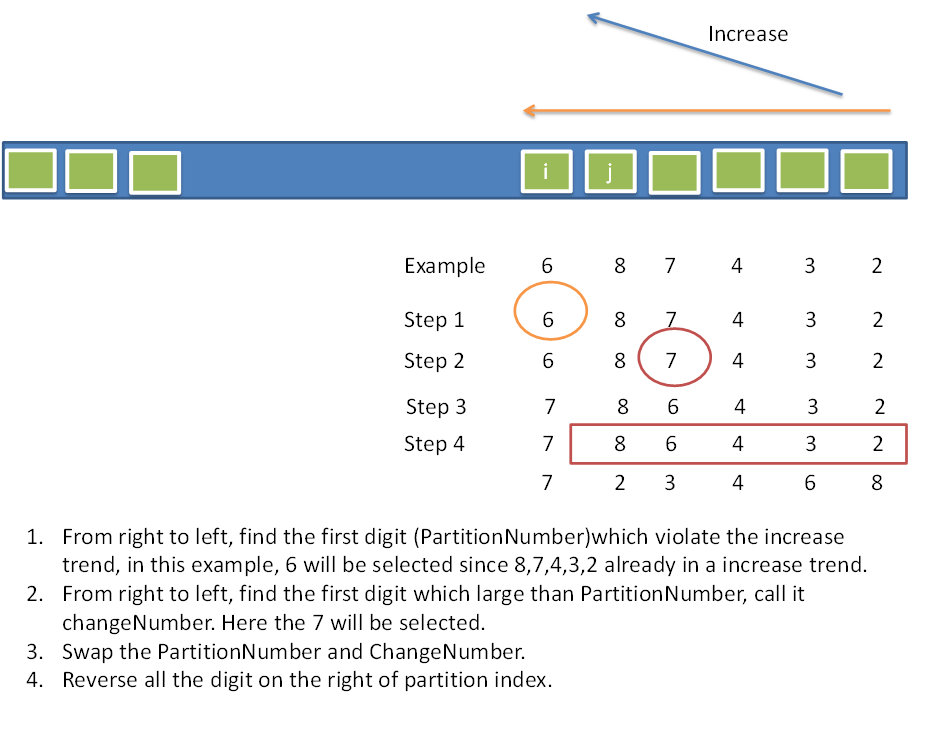
\includegraphics[width=360pt]{next-permutation.png}\\
\figcaption{下一个排列算法流程}\label{fig:permutation}
\end{center}


\subsubsection{代码}
\begin{Code}
// LeetCode, Permutations
// 重新实现 next_permutation()
class Solution {
public:
    vector<vector<int>> permute(vector<int>& num) {
        sort(num.begin(), num.end());

        vector<vector<int>> permutations;

        do {
            permutations.push_back(num);
        } while (next_permutation(num.begin(), num.end()));

        return permutations;
    }

    template<typename BidiIt>
    bool next_permutation(BidiIt first, BidiIt last) {
        // Get a reversed range to simplify reversed traversal.
        const auto rfirst = reverse_iterator<BidiIt>(last);
        const auto rlast = reverse_iterator<BidiIt>(first);

        // Begin from the second last element to the first element.
        auto pivot = next(rfirst);

        // Find `pivot`, which is the first element that is no less than its
        // successor.  `Prev` is used since `pivort` is a `reversed_iterator`.
        while (pivot != rlast and !(*pivot < *prev(pivot)))
            ++pivot;

        // No such elemenet found, current sequence is already the largest
        // permutation, then rearrange to the first permutation and return false.
        if (pivot == rlast) {
            reverse(rfirst, rlast);
            return false;
        }

        // Scan from right to left, find the first element that is greater than
        // `pivot`.
        auto change = find_if(rfirst, pivot, bind1st(less<int>(), *pivot));

        swap(*change, *pivot);
        reverse(rfirst, pivot);

        return true;
    }
};
\end{Code}


\subsection{深搜}
本题是求路径本身,求所有解,函数参数需要标记当前走到了哪步,还需要中间结果的引用,最终结果的引用。

扩展节点,每次从左到右,选一个没有出现过的元素。

本题不需要判重,因为状态装换图是一颗有层次的树。收敛条件是当前走到了最后一个元素。

\subsubsection{代码}
\begin{Code}
// LeetCode, Permutations
// 深搜
class Solution {
public:
    vector<vector<int> > permute(vector<int>& num) {
        sort(num.begin(), num.end());

        vector<vector<int>> result;
        vector<int> p(num.size(), 0);  // 中间结果

        permute(num.begin(), num.end(), 0, p, result);
        return result;
    }
private:
    typedef vector<int>::const_iterator Iter;
    void permute(Iter first, Iter last, int cur, vector<int> &p,
            vector<vector<int> > &result) {
        if ((first + cur) == last) {  // 收敛条件
            result.push_back(p);
        }

        // 扩展状态
        for (auto i = first; i != last; i++) {
            bool used = false;
            // 查找 *i 是否在p[0, cur) 中出现过
            for (auto j = p.begin(); j != p.begin() + cur; j++) {
                if (*i == *j) {
                    used = true;
                    break;
                }
            }
            if (!used) {
                p[cur] = *i;
                permute(first, last, cur + 1, p, result);
                // 不需要恢复P[cur],返回上层cur会自动减1,P[cur]会被覆盖
            }
        }
    }
};
\end{Code}


\subsubsection{相关题目}
\begindot
\item Permutations II ,见 \S \ref{sec:permutations-ii}
\myenddot


\section{Permutations II} %%%%%%%%%%%%%%%%%%%%%%%%%%%%%%
\label{sec:permutations-ii}


\subsection{next_permutation()}
上一题中的代码,见\S \ref{sec:next-permutation} 节,也适用于本题。


\subsection{重新实现next_permutation()}
上一题中的代码,见\S \ref{sec:next-permutation-implement} 节,也适用于本题。


\subsection{深搜}
递归函数\fn{permute()}的参数\fn{p},是中间结果,它的长度又能标记当前走到了哪一步,用于判断收敛条件。

扩展节点,每次从小到大,选一个没有被用光的元素,直到所有元素被用光。

本题不需要判重,因为状态装换图是一颗有层次的树。


\subsubsection{代码}
\begin{Code}
// LeetCode, Permutations II
// 深搜
class Solution {
public:
    vector<vector<int> > permuteUnique(vector<int>& num) {
        sort(num.begin(), num.end());

        unordered_map<int, int> count_map; // 记录每个元素的出现次数
        for_each(num.begin(), num.end(), [&count_map](int e) {
            if (count_map.find(e) != count_map.end())
                count_map[e]++;
            else
                count_map[e] = 1;
        });

        // 将map里的pair拷贝到一个vector里
        vector<pair<int, int> > elems;
        for_each(count_map.begin(), count_map.end(),
                [&elems](const pair<int, int> &e) {
                    elems.push_back(e);
                });

        vector<vector<int>> result; // 最终结果
        vector<int> p;  // 中间结果

        n = num.size();
        permute(elems.begin(), elems.end(), p, result);
        return result;
    }

private:
    size_t n;
    typedef vector<pair<int, int> >::const_iterator Iter;

    void permute(Iter first, Iter last, vector<int> &p,
            vector<vector<int> > &result) {
        if (n == p.size()) {  // 收敛条件
            result.push_back(p);
        }

        // 扩展状态
        for (auto i = first; i != last; i++) {
            int count = 0; // 统计 *i 在p中出现过多少次
            for (auto j = p.begin(); j != p.end(); j++) {
                if (i->first == *j) {
                    count ++;
                }
            }
            if (count < i->second) {
                p.push_back(i->first);
                permute(first, last, p, result);
                p.pop_back(); // 撤销动作,返回上一层
            }
        }
    }
};
\end{Code}


\subsubsection{相关题目}
\begindot
\item Permutations ,见 \S \ref{sec:permutations}
\myenddot
